\chapter{FastIC+}
The FastIC+ is a configurable ASIC for fast timing applications, featuring 8-channel front-end for photo detectors such as SiPM, PMT or MCP, capable of precisely measuring the Time-of-Arrival (ToA) and Time-over-Treshold (ToT) of photons hitting the detectors. This feature set finds it's use applications that require precise photon timestamping, such as Time-of-Flight Positron Emission Tomography, high-energy physics, mass-spectrometry or LIDAR applications. The ASIC is developed in the \SI{65}{\nano\meter} technology by the Institut de Ciencies del Cosmos of the University of Barcelona in close colaboration with CERN. 


\FloatBarrier
\begin{figure}[htp!]
    \centering
    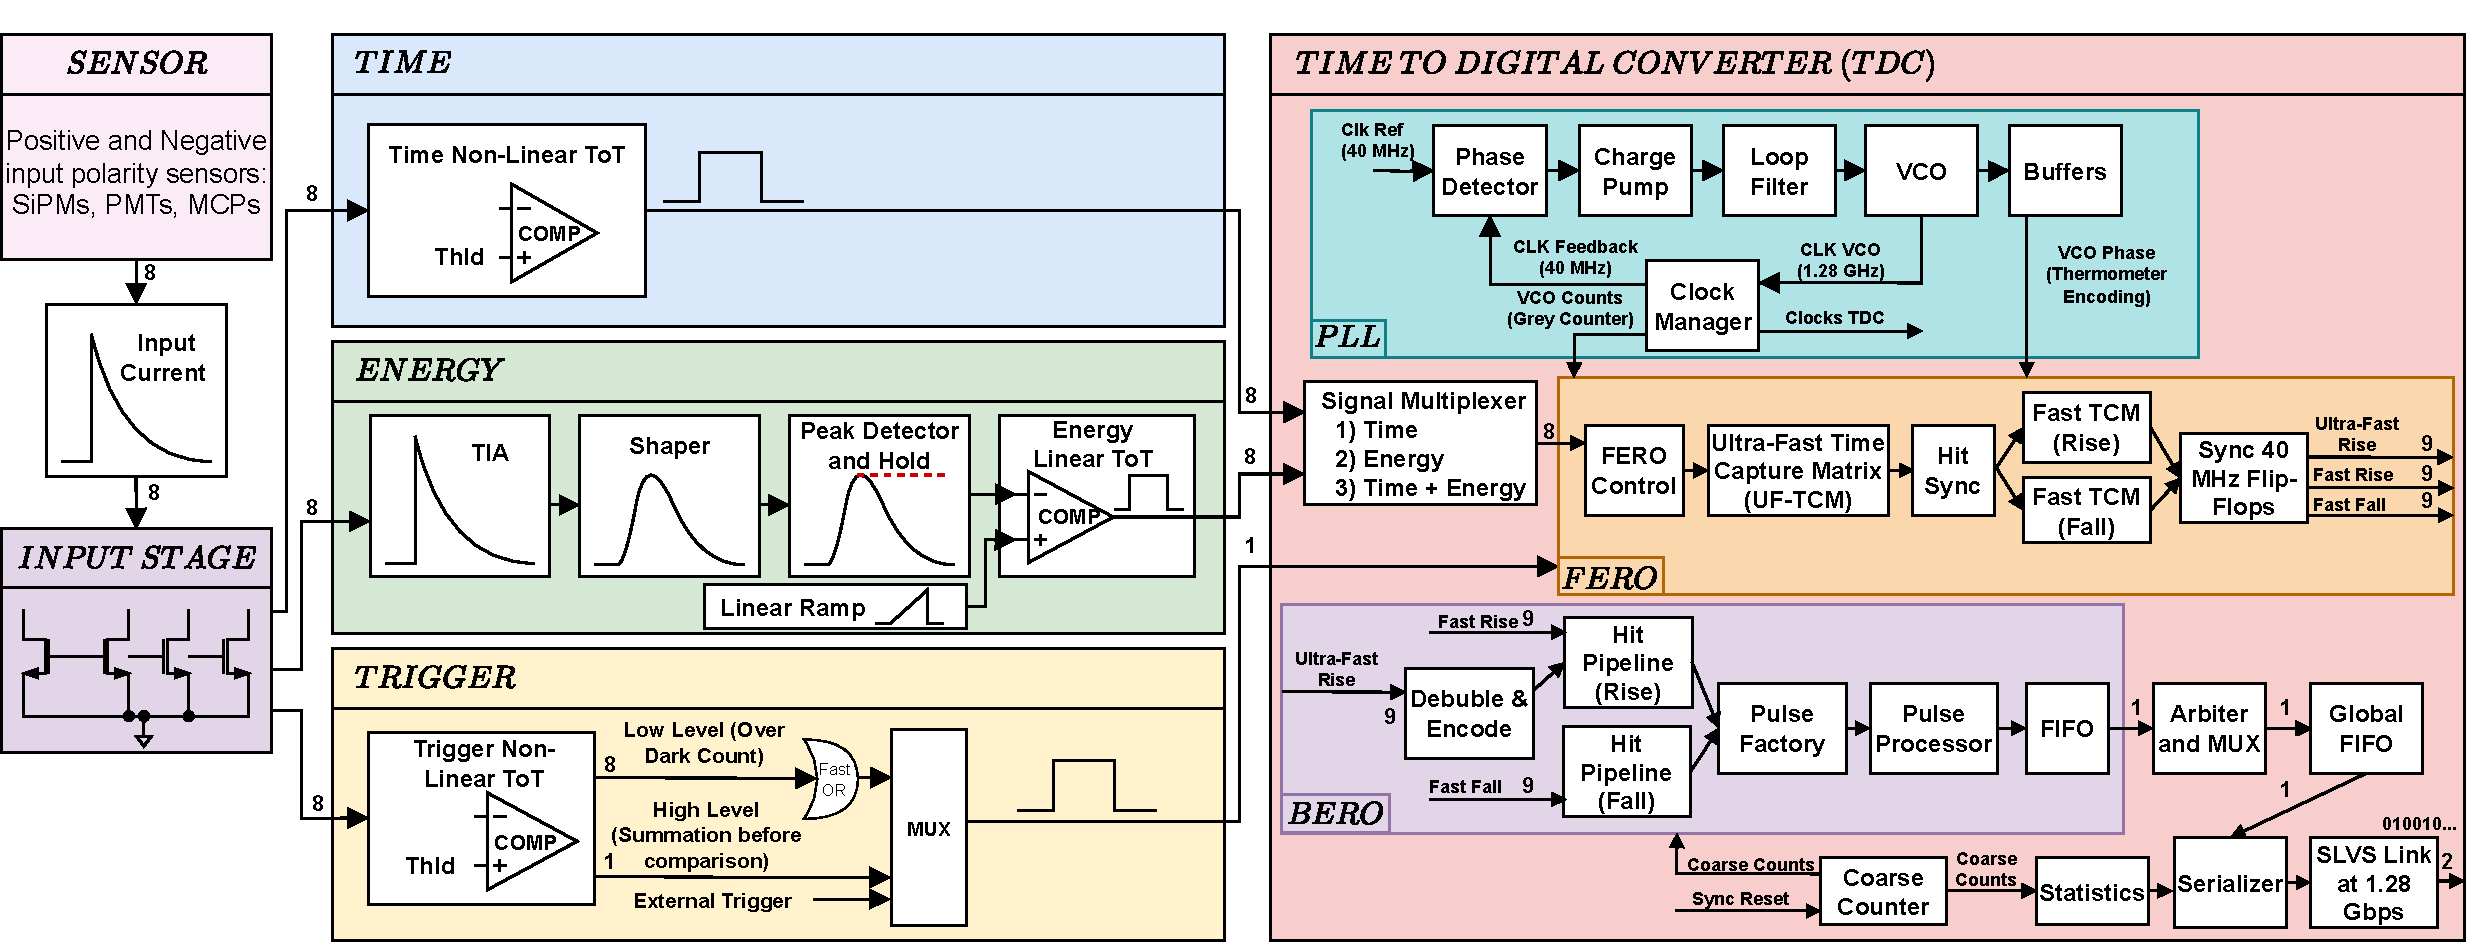
\includegraphics[height=4.8cm]{05_FASTICPLUS_BLOCK.pdf}
    \caption{Top-level architecture block diagram}
    \label{fig:fastic_top_level}
\end{figure}
\FloatBarrier



\section{Detection}
\label{sec:fastic:detection}

Each channel consists of a low impedance input stage, working with both positive and negative polarity sensors with dynamic range of \SI{5}{\micro\ampere} to \SI{20}{\milli\ampere} and stability across sensor capacitances from \SI{10}{\pico\farad} to \SI{1}{\nano\farad}, which generates three differently scaled replicas of the input current pulse and forwards it over the three signal paths: time, energy and trigger.
%
\subsection{Time path}
The time path acts as a simple discriminator which compares the pulse to a programmable treshold, which can be set down to a single photoelectron level. The leading edge of the comparator pulse provides the ToA timestamp and the OR of all channels can be output via the \verb|TIME| output. 
%
\subsection{Energy path}
The energy path extraxts the pulse peak in order to estimate the energy deposited in the sensor. The chain consists of a transimpedance amplifier, shaper, peak detector with hold and a comparator that compares the peak detector level with a linear ramp. The length of tha output pulse than directly provides the energy ef the pulse. The input can also be compared to a constant treshold to provide a non-linear ToT instead. 

\subsection{Trigger path}
The last, trigger, path generates either a low-level trigger per every channel or a cluster trigger. The low-level trigger is an OR of all the trigger comparators for all channels whereas the cluster trigger results from a analog summation of the input pulses passed through a single comparator. This trigger can be used internally to trigger the conversion FSM, output on a pin or an external trigger can be provided on a pin aswell.

%Three different measurement modes, 
%\begin{itemize}
%    \item ToA (non-linear ToT),
%    \item Energy (from ToT),
%    \item Hybrid (ToA + Energy),
%\end{itemize}
%are present to allow the user to optimize for measurement of ToA, ToT or both. The maximum detection rate of the impacts is approximately \SI{2}{\mega\hertz} in the linear mode and \SI{50}{\mega\hertz} in non-linear mode.


\section{Digitizing}
The time, energy and trigger pulses from each channel is than passed to a Front-End Readout block (FERO) which interpolates the input pulse and obtains a digital representation of the rising (with a \SI{25}{\pico\second} time bin) and falling (with a \SI{390}{\pico\second} time bin) edges.

After the edge capture, the timing information is passed to the Back-End Readout Block (BERO) which processes the information. It corrects any signal errors, performs trigger validation and filering and encodes the timing information into a suitable binary format. In the end, it stores the encoded packet in a FIFO buffer. Arbiter with a MUX than handles the requests from all the channels and stores the packets in a global FIFO. 

As a laste step, a Aurora serializer converts the packets from the FIFO into a Aurora 64B/66B serial stream and sends it over the high speed output lines. The stream speed can be configured at speeds from \SI{80}{\mega\bit\per\second} to \SI{1.28}{\giga\bit\per\second} in the accordance with the Aurora specification.


%\section{Configuration and testing}
%An I2C interface has been implemented alongside the Aurora bus to allow for easy configuration of the chip parameters. This interface can run at speeds up to \SI{1}{\mega\hertz} and can be shared between multiple FastIC+ chips. 

%For testing purposes, four debug pins are exposed to read out the state of the internal FSM. If not used for debugging, they can be utilized for configuration of the I2C address. 
